\chapter{Architecture}
\label{sec:architecture}

The system has three parts: a data collection environment, an offline
training pipeline, and a live prober. Data collection and training run once
(or whenever new data is needed) and produce static model files. The prober
is what runs in production. Chapter~\ref{chapter:implementation} covers the
source code and configuration details, this chapter describes how the parts
fit together.

% =============================================================================
\section{System Overview}
\label{sec:system-overview}

Figure~\ref{fig:system-pipeline} shows the end-to-end flow.

\begin{figure}[htbp]
  \centering
  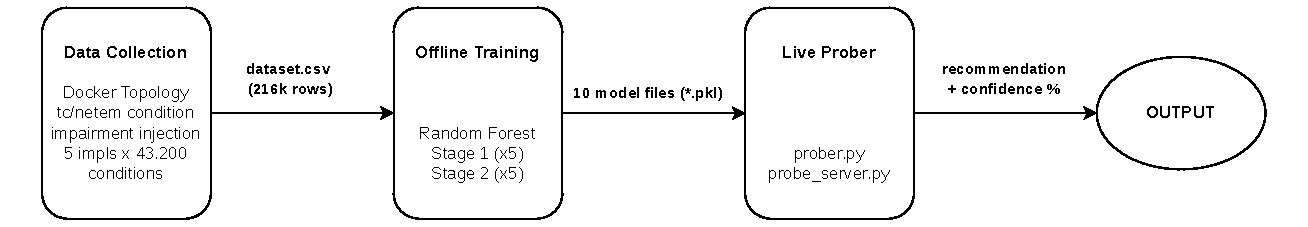
\includegraphics[width=\textwidth]{src/img/arch/fig_system_pipeline.pdf}
  \caption{End-to-end system overview. Data collection produces a CSV dataset
           that feeds offline training. The trained models are loaded by the
           live prober, which measures network conditions and outputs a
           recommendation.}
  \label{fig:system-pipeline}
\end{figure}

The prober does not retrain or update anything at runtime. It loads the
trained models from disk and runs inference in under a second. Everything
computationally expensive happens offline.

% =============================================================================
\section{Test Topology}
\label{subsec:topology}

Data collection runs inside a Docker Compose setup of four containers: the
client, the server, the simulator that connects them, and a dedicated iperf3
target that absorbs optional competing traffic. Figure~\ref{fig:topology} shows
the layout.

\begin{figure}[htbp]
  \centering
  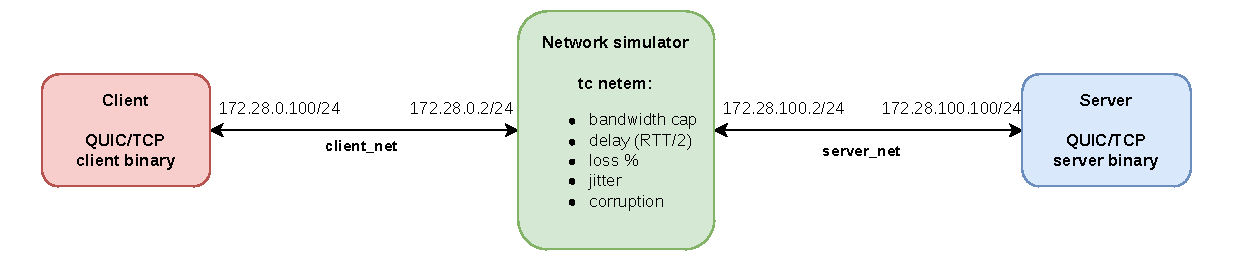
\includegraphics[width=\textwidth]{src/img/arch/fig_topology.pdf}
  \caption{Docker Compose test topology. Each container runs in
           its own network namespace, shown with a distinct background colour.
           The two Docker bridge networks, \texttt{client\_net} (172.28.0.0/24)
           and \texttt{server\_net} (172.28.100.0/24), are separate layer-2
           segments. Every container attaches to a bridge through a veth pair.
           The simulator is a single namespace with one interface on each bridge
           (\texttt{eth0} at 172.28.0.2/24, \texttt{eth1} at 172.28.100.2/24) and
           is the only forwarding path between the endpoints, applying
           \texttt{tc netem} impairments on both legs. The iperf3 target
           (172.28.0.200/24 on \texttt{client\_net}, shown dashed) is the sink
           for the optional competing traffic the simulator generates. The
           competing traffic egresses through the same \texttt{eth0} netem qdisc
           as the server-to-client application data, so it contends on the same
           bottleneck.}
  \label{fig:topology}
\end{figure}

The client lives on \texttt{client\_net} (172.28.0.0/24) and the server on
\texttt{server\_net} (172.28.100.0/24). The simulator is attached to both:
172.28.0.2 toward the client, 172.28.100.2 toward the server. Each container is
a separate network namespace: the simulator holds two veth interfaces, one on
each bridge, rather than belonging to both networks as a single shared entity.
Static routes are added at container startup so all traffic between client and
server goes through the simulator. Neither side can reach the other directly.

A fourth container, the iperf3 target, sits on \texttt{client\_net} at
172.28.0.200, which has no part in the application transfer under test. The container's
only job is to receive the competing TCP or UDP streams that the simulator optionally
generates with iperf3. Because that traffic leaves the simulator through
\texttt{eth0}, it crosses the same netem qdisc as the real server-to-client data
and competes with it for the shaped bandwidth, approximating cross-traffic on a
shared bottleneck link. When competing traffic is disabled, the target sits idle.

Impairments are configured with \texttt{tc netem} on the simulator's egress
interfaces, meaning every packet in either direction crosses a netem qdisc.
The same netem qdisc also caps the bandwidth through its built-in \texttt{rate}
parameter, so a single qdisc handles both shaping and impairment. One run fixes
all seven condition parameters for the duration of a single transfer, then
the containers reset for the next condition.

% =============================================================================
\section{Recommender Pipeline}
\label{subsec:recommender-pipeline}

The recommender is a two-stage classification pipeline.
Figure~\ref{fig:ml-pipeline} shows the structure.

\begin{figure}[htbp]
  \centering
  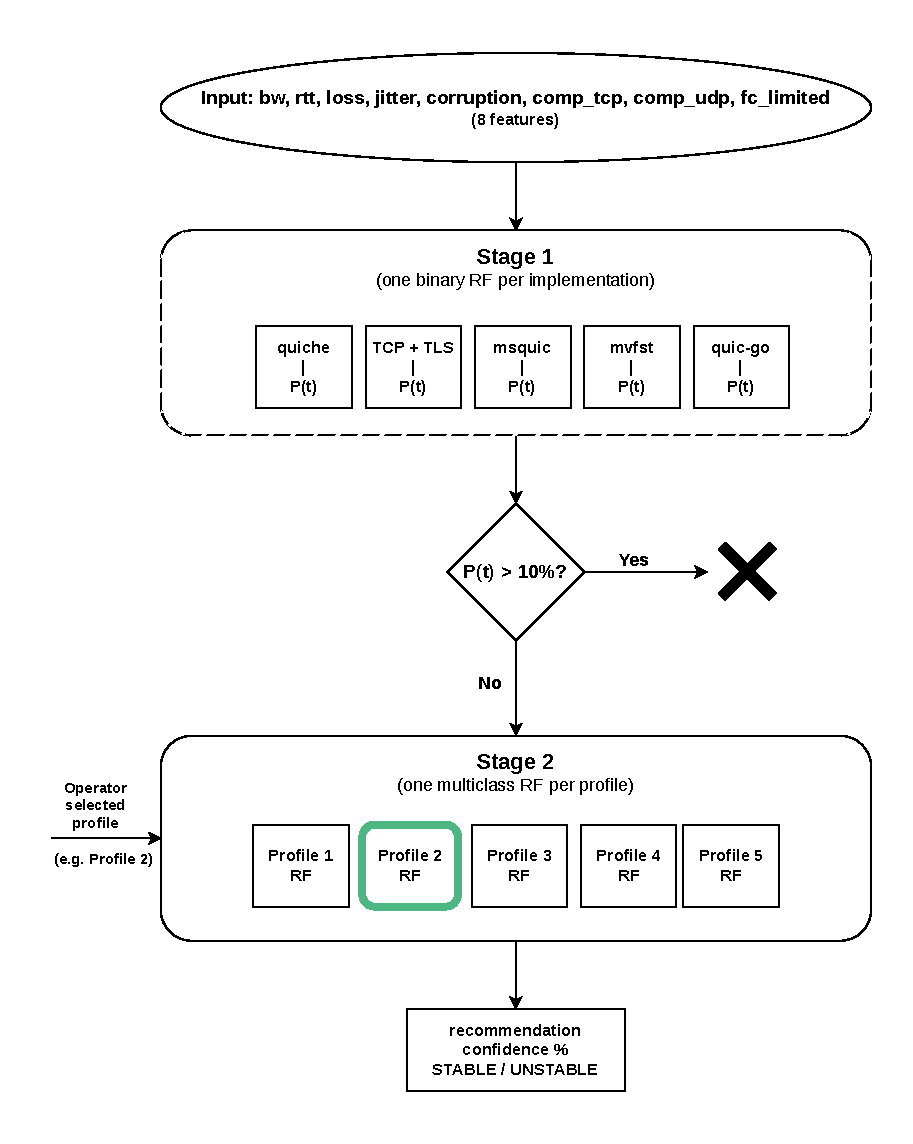
\includegraphics[width=\textwidth]{src/img/arch/fig_ml_pipeline.pdf}
  \caption{Two-stage recommender pipeline. Stage~1 runs one binary
           classifier per implementation to estimate timeout risk.
           Those above the 10\% threshold are eliminated. Stage~2 runs
           a profile-specific multiclass classifier over the survivors
           and returns a ranked recommendation with a confidence score.}
  \label{fig:ml-pipeline}
\end{figure}

Stage~1 has five binary Random Forests, one per implementation. Each takes
the same 8-feature input and outputs a timeout probability. Implementations
above the 10\% threshold are dropped and do not reach Stage~2. The threshold
is configurable at inference time.

Stage~2 has five multiclass Random Forests, one per profile. Only the one
matching the operator's selected profile runs. It takes the same input and
outputs a probability distribution over the surviving implementations. The
highest-probability class is the recommendation: that probability is the
confidence. If confidence is below 60\%, the result is flagged UNSTABLE,
meaning two or more implementations are too close to separate reliably from
the available measurements.

The two stages are trained independently. Stage~1 uses binary timeout labels
from raw run data. Stage~2 uses composite profile scores computed from
per-condition averaged metrics. Both use 5-fold GroupKFold cross-validation
at the condition level to prevent leakage between repetitions of the same
condition.

% =============================================================================
\section{Prober Deployment}
\label{sec:prober}

The prober is the production-facing part of the system. It runs on the
client, coordinates a short burst of test transfers with a counterpart on
the server, measures the resulting conditions, and runs both pipeline stages.

There are two deployment modes. In \textbf{cooperative mode}, a lightweight
\texttt{probe\_server.py} process runs on the server side. The prober sends
several measurement rounds (default: 3), receives per-implementation
throughput and timing samples, averages across rounds, and feeds the result
to the classifiers. This is the mode used in all experiments in this thesis.

In \textbf{passive mode}, no server-side process is needed. The prober estimates
bandwidth with a short iperf3 burst and measures RTT with ICMP pings against
any reachable endpoint. Passive mode is less accurate, especially for loss
and corruption, but works against existing services without any coordination.

The output is the same in both modes: Stage~1 timeout probabilities per
implementation (with eliminated ones marked), the Stage~2 recommendation for
the chosen profile, a confidence percentage, and a STABLE/UNSTABLE flag.
